There's a lot of information on diseases in the book Clinical Neuroscience,
sounds like a good place to start


\chapter{Magnetic Resonance Imaging: A Non-invasive Study of Brain's Anatomy, Connectivity and Function}
\label{ch:bkgrnd}

Este cap\'itulo est\'a basado en el libro \textit{Diffusion MRI} 
\cite{Basser2009} y en las clases del Doctor Michael L. Lipton 
\cite{Lipton2014} disponibles online. En caso de querer profundizar en 
alg\'un tema, por favor referirse a estos. 

\section{Imagen por resonancia magnética}
Se denomina momento magn\'etico nuclear al momento magn\'etico que posee
un \'atomo a causa del $spin$ de sus protones y electrones. Cuando un 
prot\'on con momento magn\'etico $\vec{\mu}$ es puesto dentro de un campo
magn\'etico comenzar\'a a preceder en torno a la direcci\'on de este
\'ultimo con una frecuencia: 

$$ \omega = \vec{\mu} \times \vec{B} = \gamma \vec{J} \times B $$

Esta es la frecuencia de Larmor, donde $\omega$ es la velocidad angular;
$\gamma$ es la relaci\'on giromagn\'etica del prot\'on; $\vec{J}$ es su
momento angular y $B$ es la fuerza del campo. A su vez, la cantidad de
energ\'ia del campo determinar\'a el \'angulo entre el momento magn\'etico
$\vec{\mu}$ y el campo $\vec{B}$ mientras sucede la precesi\'on (figura
\ref{fig:nosignal}). Esto quiere decir que dado un $B$ suficientemente
grande es posible hacer que la precesi\'on suceda en la direcci\'on
transversal del campo, lo cual permitir\'ia medir $|\mu|$ simplemente
poniendo una bobina en ese plano (figura \ref{fig:signal}). Si uno
realizara el experimento y midiera $|\mu|$ utilizando la bobina notar\'ia
que al apagar el campo, la se\~nal comienza a desvanecerse. Esto es porque
el sistema comienza a perder energ\'ia provocando que el \'angulo entre 
$\mu$ y el campo se achique. A este proceso se lo denomina relajaci\'on. \\

\begin{figure}[h!]

\begin{minipage}[b]{0.49\textwidth}
    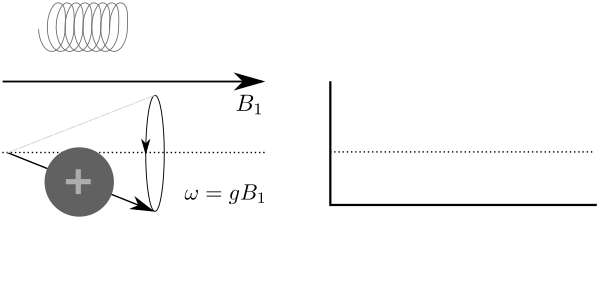
\includegraphics[width=\textwidth]{2.background/dmri/img/spin0.png}
    \caption{$Spin$ sometido a un campo magn\'etico debil. La bobina no
             detecta el prot\'on.}
    \label{fig:nosignal}
\end{minipage} ~ %add desired spacing between images, e. g. ~, \quad, \qquad, \hfill etc. %(or a blank line to force the subfigure onto a new line) 
\hfill
\begin{minipage}[b]{0.49\textwidth}
    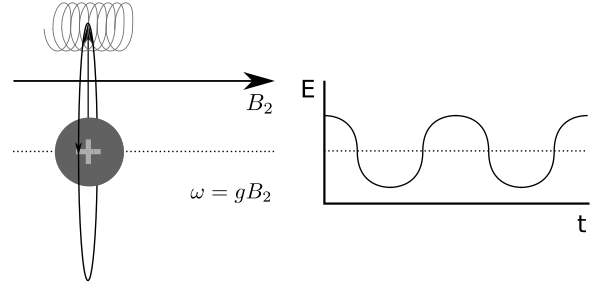
\includegraphics[width=\textwidth]{2.background/dmri/img/spin1.png}
    \caption{Resultado de aumentar el campo magn\'etico. La bobina 
             detecta el prot\'on.}
    \label{fig:signal}    
\end{minipage} ~ %add desired spacing between images, e. g. ~, \quad, \qquad, \hfill etc. %(or a blank line to force the subfigure onto a new line) 

\end{figure}

Vayamos ahora al plano m\'edico. El cuerpo est\'a compuesto por distintos 
tipos de tejidos, cada uno con su propia composici\'on qu\'imica. Esto 
determina un momento magn\'etico distinto para cada uno de ellos y por
ende, un tiempo de relajaci\'on particular. Supongamos se pone una persona
dentro de un campo magn\'etico. Cada uno de sus tejidos comenzar\'a a 
generar un momento en base a la poblaci\'on de protones que posea. 
Una forma de medir el tiempo de relajaci\'on de cada tejido ser\'ia
trasladando la precesi\'on al plano transversal. Si uno administrara 
la energ\'ia necesaria para esto simplemente aumentando la fuerza del
campo magn\'etico
da\~nar\'ia al paciente. Aqu\'i es donde se aprovecha fuertemente la
frecuencia de Larmor. Conociendo la composici\'on qu\'imica de cada tejido
es posible calcular de antemano su frecuencia angular. Luego, mediante el
efecto de resonancia es posible transmitir energ\'ia al sistema
simplemente emitiendo ondas en esa misma frecuencia. \\

\begin{figure}[h!]
                                                                                                                        
\begin{minipage}[b]{0.49\textwidth}
    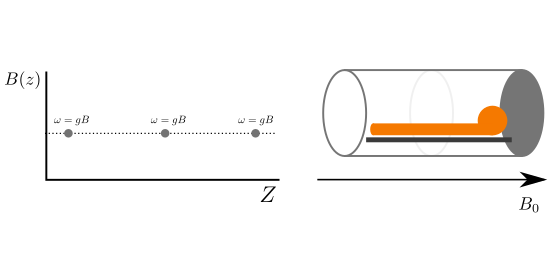
\includegraphics[width=\textwidth]{2.background/dmri/img/grad0.png}
    \caption{\small  Campo uniforme, todos los protones poseen la misma velocidad angular.}
     \label{fig:unif}
\end{minipage} ~
\hfill
\begin{minipage}[b]{0.49\textwidth}
    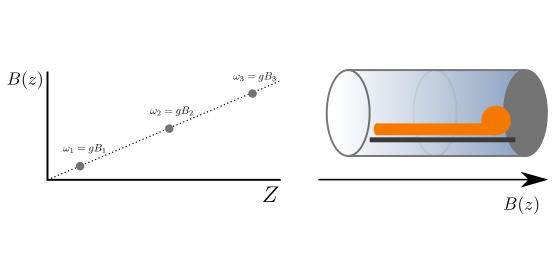
\includegraphics[width=\textwidth]{2.background/dmri/img/grad1.png}
    \caption{\small Campo gradiente, la velocidad angular de los protones var\'ia linealmente. }
    \label{fig:grad}
\end{minipage} ~

\end{figure}  


Los resonadores magn\'eticos son dispositivos con la capacidad de generar 
campos y pulsos en diferentes frecuencias. En particular todo resonador
encendido est\'a emitiendo constantemente un campo homog\'eneo $B_0$
(figura \ref{fig:unif}). El problema entonces es: ¿C\'omo obtener el tiempo
de relajaci\'on de un punto particular del cuerpo? Una respuesta posible
es utilizar campos gradientes. Un campo gradiente es un campo que var\'ia
su potencia linealmente a lo largo de una direcci\'on, provocando que todas
los protones a lo largo de dicha direcci\'on var\'ien su frecuencia
angular de manera predecible. Aplicando un campo gradiente $G_z$ en la
direcci\'on $z$ (figura \ref{fig:grad}) sobre la persona haremos que la
velocidad en funci\'on de la posici\'on sea: $\omega(z) = B_z(z) g$, esto
nos asegurara que si aplicamos un pulso de radio frecuencia (RF) con una
frecuencia de $B_z(z_o) g$, solo los protones que se encuentran en la
posici\'on $z=z_o$ comenzar\'an a resonar, por lo que \'estos ser\'an los
\'unicos que generen un campo transversal. Cabe destacar que como no es
posible generar un pulso con exactamente la frecuencia deseada, tambi\'en
resonar\'an los protones que se encuentren cerca, por lo que tendremos un
intervalo $[z_o-\epsilon,z_o+\epsilon]$ resonando. A este proceso se lo
denomina \textit{slice selection}. Podemos pensar el $slice$ como una
matriz
de dos dimensiones sobre el eje $z$. Si ahora aplicamos un campo gradiente
$G_\psi$ en la direcci\'on $y$, suceder\'a que todas las  filas de nuestra
matriz adquirir\'an diferentes velocidades angulares. Al apagar $G_\psi$
todos los protones volver\'an a preceder respecto al campo $B_0$, pero est\'a
vez estar\'an desfasados por filas (figura \ref{fig:kspace}). Encendiendo 
\'un tercer campo gradiente $G_\upsilon$ sobre la direcci\'on $x$
conseguiremos que cada columna posea una frecuencia distinta y cada fila
una fase distinta. Repitiendo este procedimiento varias veces cambiando
solo la intensidad de $G_\psi$ podemos armar lo que se conoce como 
\textit{k-space}. El \textit{k-space} es una imagen espacial temporal
donde est\'an anotados los valores obtenidos para cada potencia utilizada,
en orden ascendente de potencia. El aplicar una transformada de Fourier 3D
a dicho espacio nos devolver\'a la imagen que representa el contraste de
cada tejido en el \textit{slice} seleccionado. \\

\begin{figure}[h!]
                                                                                                                        
\begin{minipage}[b]{\textwidth}
    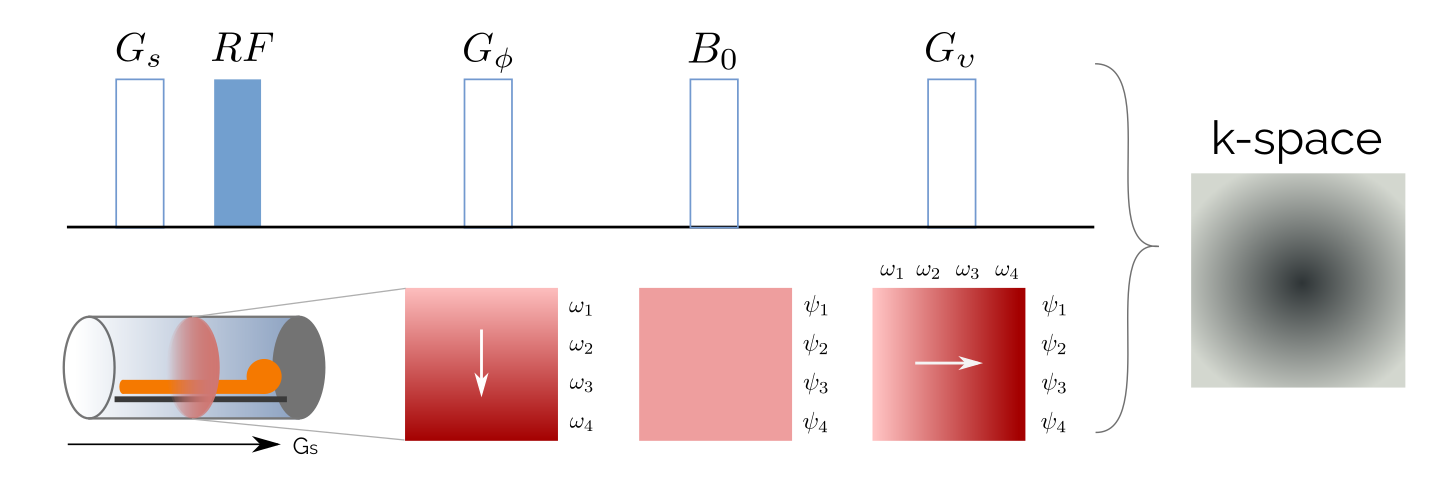
\includegraphics[width=\textwidth]{2.background/dmri/img/kspace.png}
    \caption{Resumen del proceso de adquisici\'on de im\'agenes en MRI.}
    \label{fig:kspace}
\end{minipage} ~

\end{figure}  



\section{Resonancia magn\'etica de difusi\'on}

Las mol\'eculas dentro de un fluido en equilibrio no se encuentran 
est\'aticas, sino que se mueven de manera aleatoria. A este fen\'omeno se
lo conoce con el nombre de difusi\'on. \\

En 1946 Bloch \cite{Bloch1946} prueba que la variaci\'on de la 
magnetizaci\'on nuclear en el tiempo se puede expresar como:

$$ \frac{dM(t)}{dt} = \gamma M(t) \times B(t) 
                      - \frac{M(t) \vec{x} + M(t)\vec{y}}{T_2}
                      - \frac{(M(t)-M(0))\vec{z}}{T1} $$

Donde $\gamma$ es la relaci\'on giromagn\'etica, $B$ es la intensidad del
campo magn\'etico y T1, T2 son tiempos de relajaci\'on. Mas tarde, en
1956, H.C. Torrey \cite{Torrey1956} observa que la magnetizaci\'on 
tambi\'en se pierde por efecto de la difusi\'on y extiende la ecuaci\'on
de Bloch:

$$ \frac{dM(t)}{dt} = g M(t) \times B(t) 
                      - \frac{M(t) \vec{x} + M(t)\vec{y}}{T_2}
                      - \frac{(M(t)-M(0))\vec{z}}{T1} 
                      + \nabla \cdot D \nabla M(t) $$

Esta relaci\'on se conoce como la ecuaci\'on de Bloch-Torrey. $D$ es el tensor de difusi\'on. \\

Imaginemos el siguiente experimento: luego de aplicar el pulso RF 
agregamos un campo gradiente $G_1=G_d$ durante un tiempo $\delta$ 
peque\~no. Como ya explicamos, esto generar\'a un desfase entre los $spines$
de los protones. El aplicar $G_2=-G_d$ luego de $\Delta$ deber\'ia
provocar que los $spines$ se vuelvan a alinear. Sin embargo, los protones
que se encuentren en un fluido estar\'an sometidos al efecto de la 
difusi\'on. Esto sucede, por ejemplo, en el interior de los axones.
Dependiendo del tiempo $\delta$ los protones se habr\'an movido cierta
distancia, provocando que el campo magn\'etico los alcance en distintas 
posiciones. Por ende su velocidad angular se ver\'a afectada de manera 
distinta a la esperada si no se hubieran movido. Esto nos indica que si
hay difusi\'on entonces habr\'a un desfase en esa poblaci\'on de neutrones
(figura \ref{fig:dmri}).\\

\begin{figure}
                                                                                                                        
\begin{minipage}[b]{\textwidth}
    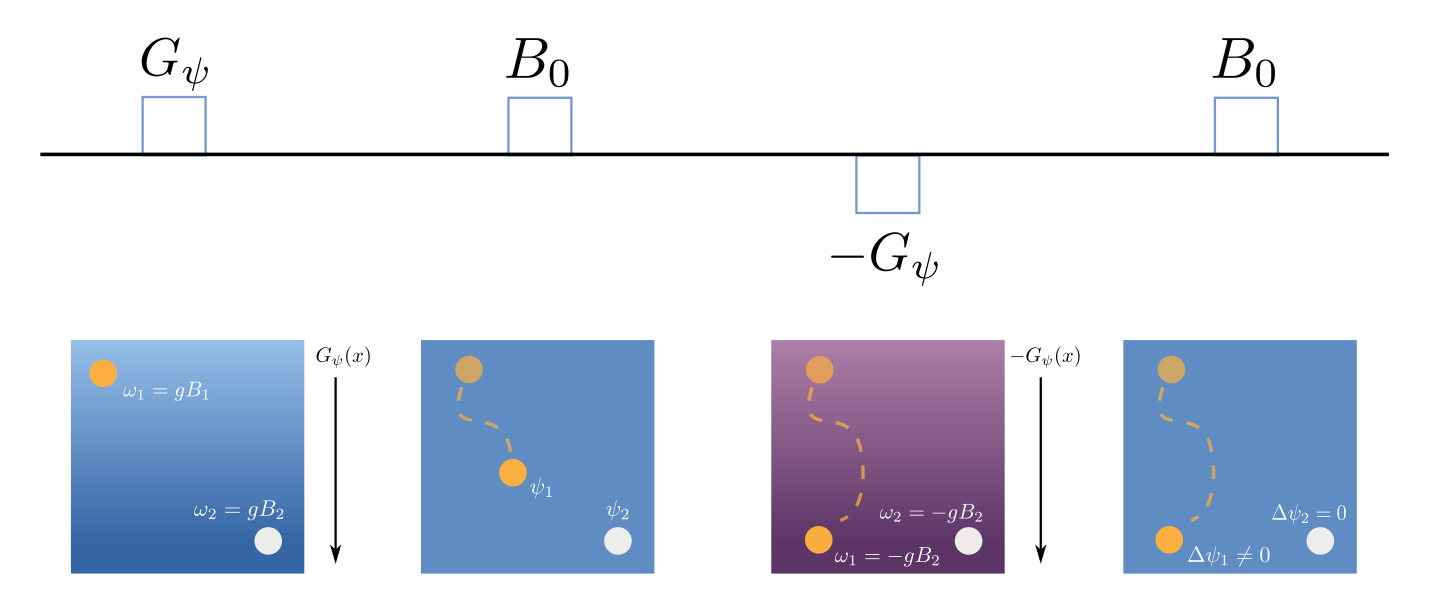
\includegraphics[width=\textwidth]{2.background/dmri/img/dmri.png}
    \caption{Modificar la secuencia de gradientes permite medir la
             intensidad de difusi\'on.}
    \label{fig:dmri}
\end{minipage} ~

\end{figure}  

La se\~nal medida en un resonador magn\'etico proviene del 
momento magn\'etico de los protones. Es importante destacar que por
limitaciones f\'isicas de los
dispositivos es imposible obtener la se\~nal producida por un
solo prot\'on. Lo que se mide es la resultante de los momentos magn\'eticos
de todos los protones dentro de un espacio. Si todos los protones est\'an
precediendo a la misma velocidad sobre el mismo plano, entonces la
resultante m\'axima se obtiene cuando todos poseen la misma fase. Esto es,
todos se encuentran en la misma posici\'on al mismo tiempo, rotando
juntos. Por ende, el desfase producto de la difusi\'on se traducir\'a en
perdida de se\~nal.\\

\begin{wrapfigure}{r}{0.5\textwidth}
    \begin{center}
        \vspace{-1cm}
        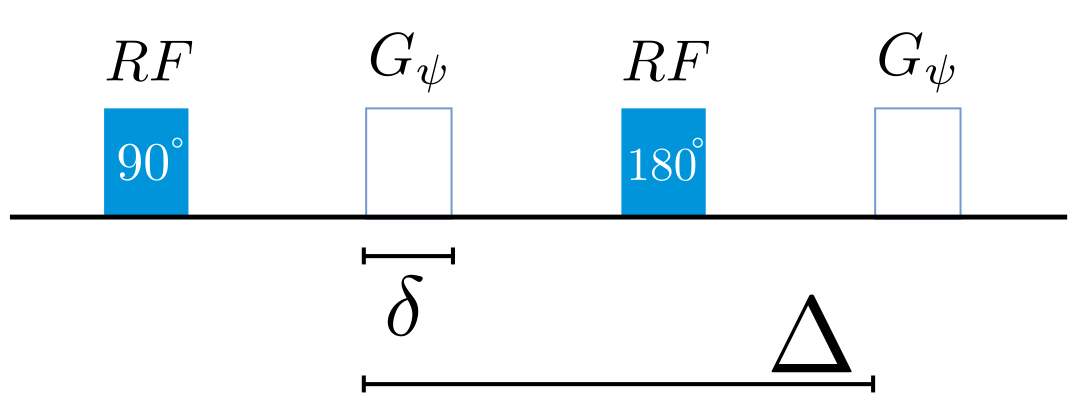
\includegraphics[width=0.4\textwidth]{2.background/dmri/img/fgp.png}
        \caption{Secuencia Pulsed Gradient Spin Echo.}
        \label{fig:fgp}
    \end{center}
\end{wrapfigure}  

En 1965 Stejskal y Tanner \cite{Stejskal1965} crean una secuencia
denominada \textit{Pulsed Gradient Spin Echo}. En la misma utilizan dos
pulsos de RF y un gradiente magn\'etico para generar un desfase entre los
protones (figura \ref{fig:fgp}). Luego demuestran que asumiendo un $\delta$
peque\~no la ecuaci\'on de Bloch-Torrey tiene soluci\'on, y la atenuaci\'on
de la se\~nal se puede expresar como:

\begin{equation}
    E(g, \delta, \Delta) = 
    \frac{S(g, \delta, \Delta)}{S_0} =
         e^{-\gamma^2 g^2 \delta^2 \left(\Delta - \frac{\delta}{3}\right) D} 
    \label{eq:st}
\end{equation}
  
Donde $E(g, \delta, \Delta)$ es la atenuaci\'on de la se\~nal obtenida; 
$g$ es la intensidad del gradiente magn\'etico; $S_0$ es la se\~nal
obtenida sin utilizar gradientes ($g=0 T/m$); $\gamma$ es la relaci\'on
giromagn\'etica del  prot\'on; $\delta$ es el tiempo que el gradiente 
est\'a encendido; $\Delta$ es el tiempo entre las activaciones del
gradiente y $D$ representa el coeficiente de difusi\'on. La raz\'on por la
cual se divide la se\~nal obtenida por $S_0$ es porque la se\~nal en cada
punto depende fuertemente de la densidad de protones que hay en el mismo,
si no ponderamos dicha densidad, es imposible comparar la intensidad de
difusi\'on en distintas regiones. \\

En 1985 Le Bihan \cite{LEBIHAN} adapta esta t\'ecnica para medir la 
difusi\'on de las part\'iculas agrupando todos los par\'ametros del
experimento dentro de un mismo par\'ametro $b$:

$$ b = \gamma^2 g^2 \delta^2 \left(\Delta - \frac{\delta}{3}\right) $$ 

Esto simplifica la ecuaci\'on \ref{eq:st} a:  

$$ E(b) = \frac{S(b)}{S_0} = e^{-b D} $$

Donde $b$ representa el reciproco de la intensidad de difusi\'on. \\

En 1994 Basser et al. \cite{Basser1994} proponen medir la atenuaci\'on de
se\~nal en distintas direcciones y luego aproximar el coeficiente de 
difusi\'on con un tensor de segundo orden. Un tensor es una matriz
multidimensional asociado a una base, que posee una ley de 
transformaci\'on  para indicar  c\'omo cambian los componentes del tensor
al cambiar de base. Esta t\'ecnica sienta las bases de lo que se conoce
como \textit{Diffusion Tensor Imaging} (DTI). En DTI el tensor m\'as
utilizado representa un elipsoide en $R^3$. La matriz que lo representa
es sim\'etrica, por ello es que se necesitan tomar al menos seis
adquisiciones: 

$$
    D =
    \begin{pmatrix}
             D_{xx} & D_{xy} & D_{xz} \\
             D_{xy} & D_{yy} & D_{yz} \\
             D_{xz} & D_{yz} & D_{zz}    
    \end{pmatrix}
$$

Uno de los principales limitantes de este m\'etodo es que no permite
representar correctamente el cruce de fibras. Esto es producto de que
caracteriza las fibras dentro de cada voxel utilizando un \'unico
elipsoide.\\

En 1991 Callaghan et al \cite{Callaghan1991} desarrollan el 
\textit{q-space analysis}. Esto permite realizar microscop\'ia mediante
dMRI. Utilizando el trabajo de Stejskal y Tanner prueban que es posible
obtener la siguiente relaci\'on entre la se\~nal atenuada y una
transformada de Fourier:

$$E(q,\Delta) =  \frac{S(q,\Delta)}{S_0} = \int_{R^2}{p(r;\Delta)e^{-2\pi i q r} dr} $$
$$ q = \frac{\gamma \delta g}{2\pi} $$

Donde $p(r;t)$ es la densidad de probabilidad de que una poblaci\'on de 
part\'iculas se desplace en direcci\'on $r$ durante un tiempo $t$. $p(r;t)$
es caracter\'istico del compartimiento donde se mueven las part\'iculas. \\

Una de las principales ventajas de \textit{q-space} sobre DTI es que no
asume ning\'un modelo a priori, esto permite definir distintos tipos de
modelos para $p(r,t)$ que caracterizan mejor el cruce de fibras. 
\textit{Spherical Harmonics} \cite{Tuch2004} o 
\textit{Constrained Spherical Deconvolution} \cite{Tournier2004}.
son ejemplos de ello.
